\documentclass{beamer} %[12pt]
\usepackage{xcolor}
%\usetheme{boadilla}
%\usetheme{malmoe}
%\usetheme{copenhagen}
%\usecolortheme{rose}
\usecolortheme{beaver}
\usepackage{pgf, graphics}
\usepackage{graphicx}
%\usepackage[left=3cm,top=3cm,right=3cm,nohead,nofoot]{geometry}
\usepackage{hyperref}
\usepackage{setspace}
\usepackage[square]{natbib}
\usepackage{amsmath}
\usepackage{amssymb}
\usepackage{verbatim}
\usepackage{color}
\usepackage{fancyvrb}
\usepackage{bbm}

\begin{filecontents}{ref.bib}
\end{filecontents}

%\usetheme{EastLansing}
%\usepackage{natbib}
\bibliographystyle{apalike}
% make bibliography entries smaller
%\renewcommand\bibfont{\scriptsize}
% If you have more than one page of references, you want to tell beamer
% to put the continuation section label from the second slide onwards
\setbeamertemplate{frametitle continuation}[from second]
% Now get rid of all the colours
\setbeamercolor*{bibliography entry title}{fg=black}
\setbeamercolor*{bibliography entry author}{fg=black}
\setbeamercolor*{bibliography entry location}{fg=black}
\setbeamercolor*{bibliography entry note}{fg=black}
% and kill the abominable icon
\setbeamertemplate{bibliography item}{}


\newcommand{\hl}[1]{\colorbox{yellow}{#1}}
\newcommand{\hlblue}[1]{\colorbox{green}{#1}}
\newcommand{\hlblu}[1]{\colorbox{cyan}{#1}}
\newcommand{\hlred}[1]{\colorbox{cyan}{#1}}
\newcommand{\hlre}[1]{\colorbox{pink}{#1}}
\newcommand{\hlgreen}[1]{\colorbox{pink}{#1}}
\newcommand{\hlgree}[1]{\colorbox{green}{#1}}



\DeclareMathOperator*{\argmax}{\arg\!\max}

\DeclareMathOperator*{\argmin}{\arg\!\min}


\newcommand{\specialcell}[2][c]{%
  \begin{tabular}[#1]{@{}c@{}}#2\end{tabular}}



%\setbeamersize{text margin left=.5cm,text margin right=.5cm}
\newenvironment{changemargin}[2]{%
  \begin{list}{}{%
    \setlength{\topsep}{0pt}%
    \setlength{\leftmargin}{#1}%
    \setlength{\rightmargin}{#2}%
    \setlength{\listparindent}{\parindent}%
    \setlength{\itemindent}{\parindent}%
    \setlength{\parsep}{\parskip}%
  }%
  \item[]}{\end{list}}
\setbeamertemplate{navigation symbols}{}%remove navigation symbols
\usepackage{color}
\newcommand{\hilight}[1]{\colorbox{yellow}{#1}}
\setbeamertemplate{footline}[page number]

\begin{document}


\title[dedup]{Today:  Using the Internet \\ Grammar of Graphics \\ 1-D Categorical \\ Friday:  ggplot2, 1-D Categorical}


\author[Samuel L. Ventura]{\\
  \large{Sam Ventura\\36-315}}
\institute[CMU Statistics]{Department of Statistics\\Carnegie Mellon University}
\date{\today}


\begin{frame}
	\maketitle
	
\end{frame}


\begin{frame}\frametitle{Via Quartz:  Who Oscar Winners Thank}
	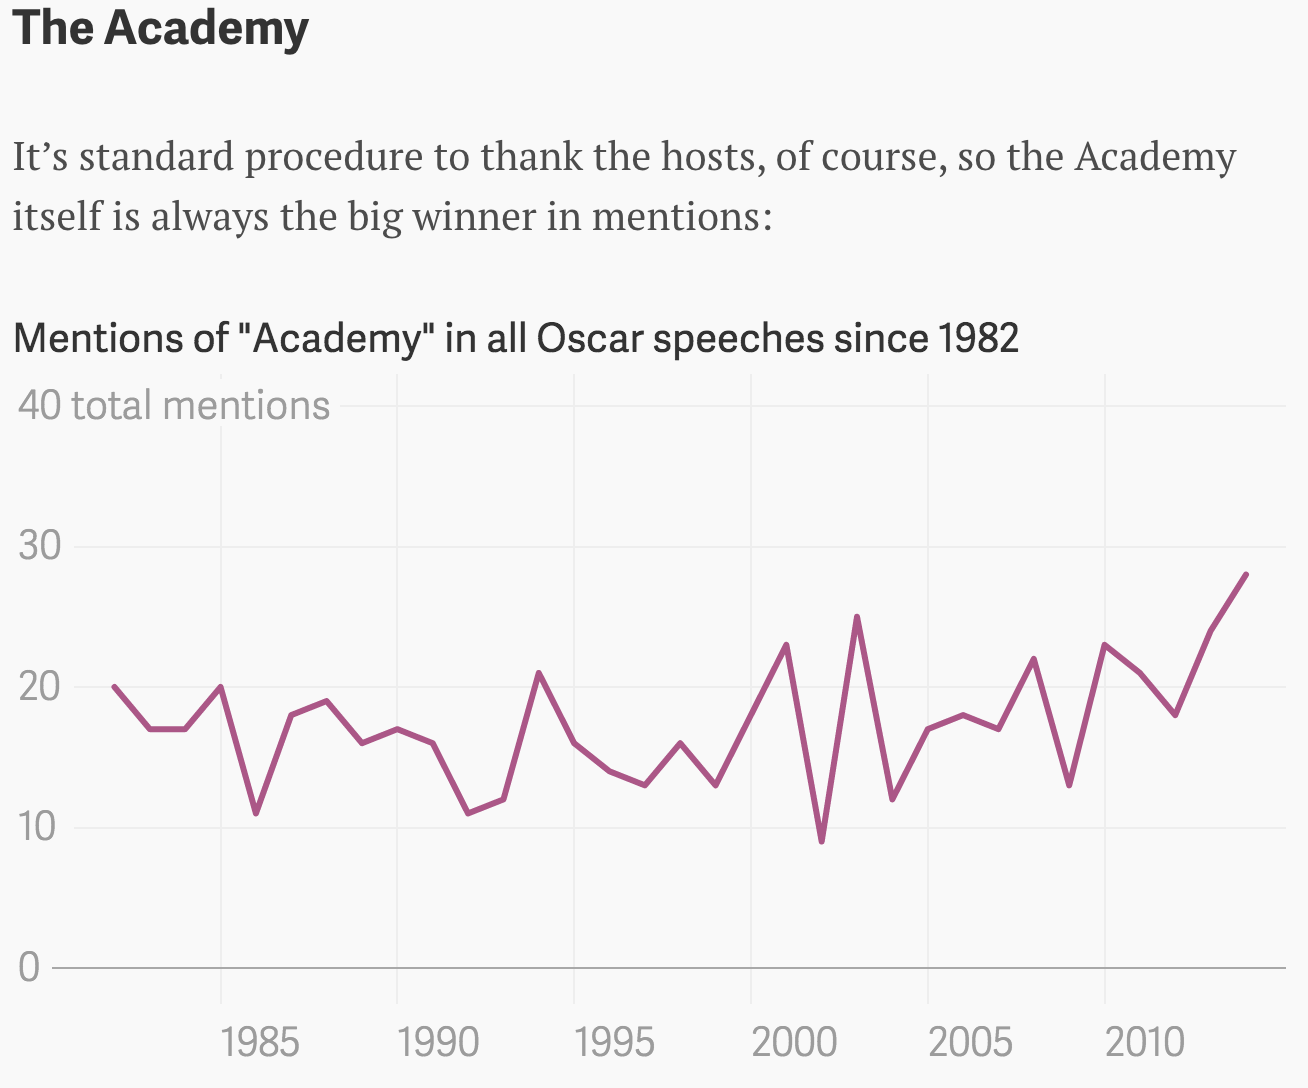
\includegraphics[width=0.7\linewidth]{academy.png}
\end{frame}

\begin{frame}\frametitle{Via Quartz:  Who Oscar Winners Thank}
	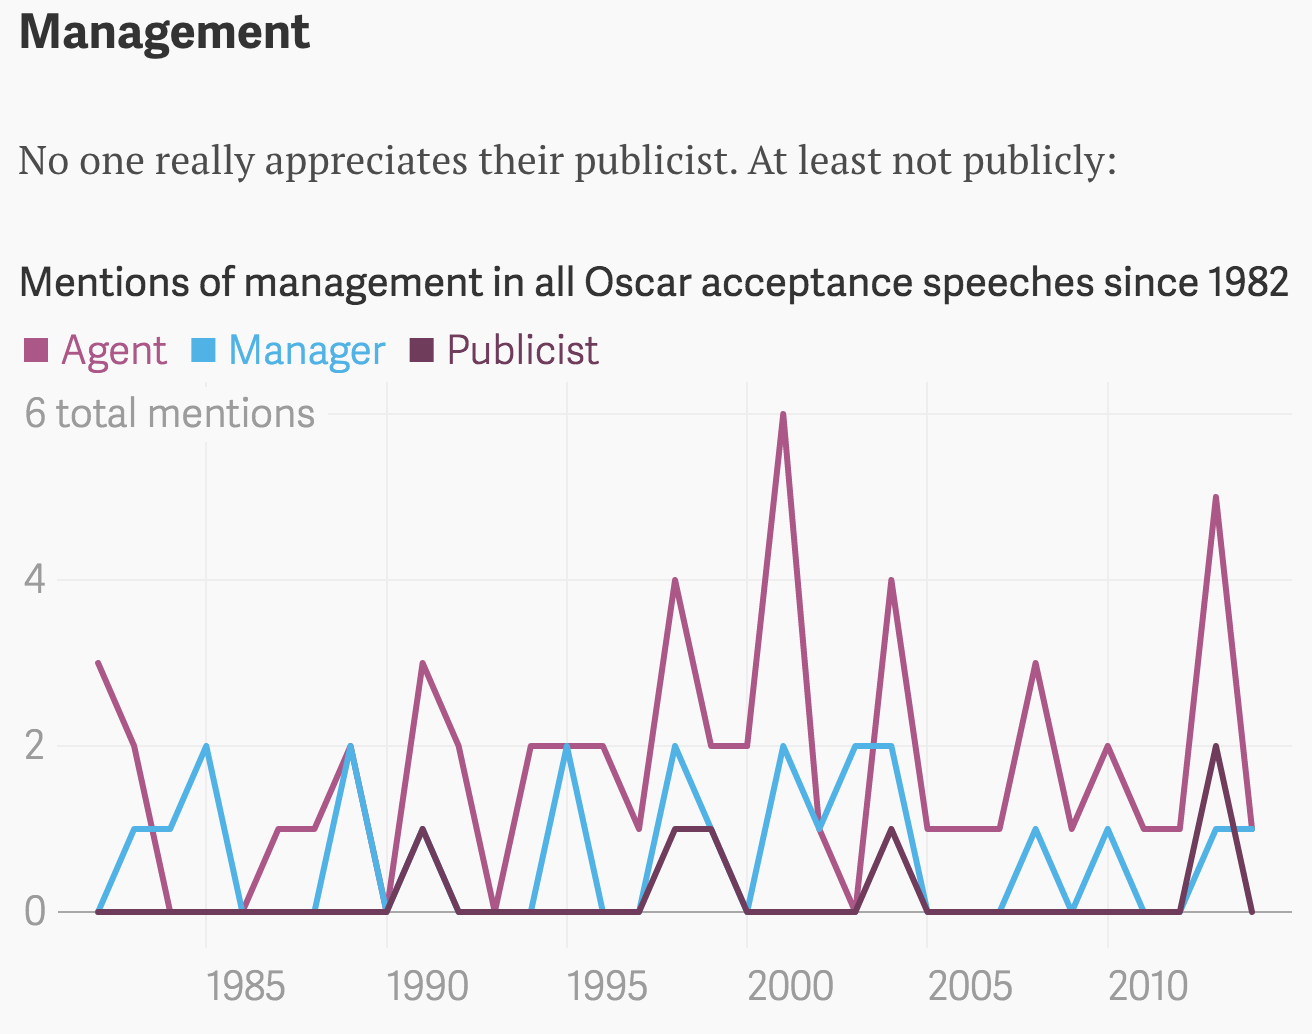
\includegraphics[width=0.7\linewidth]{management.png}
\end{frame}

\begin{frame}\frametitle{Via Quartz:  Who Oscar Winners Thank}
	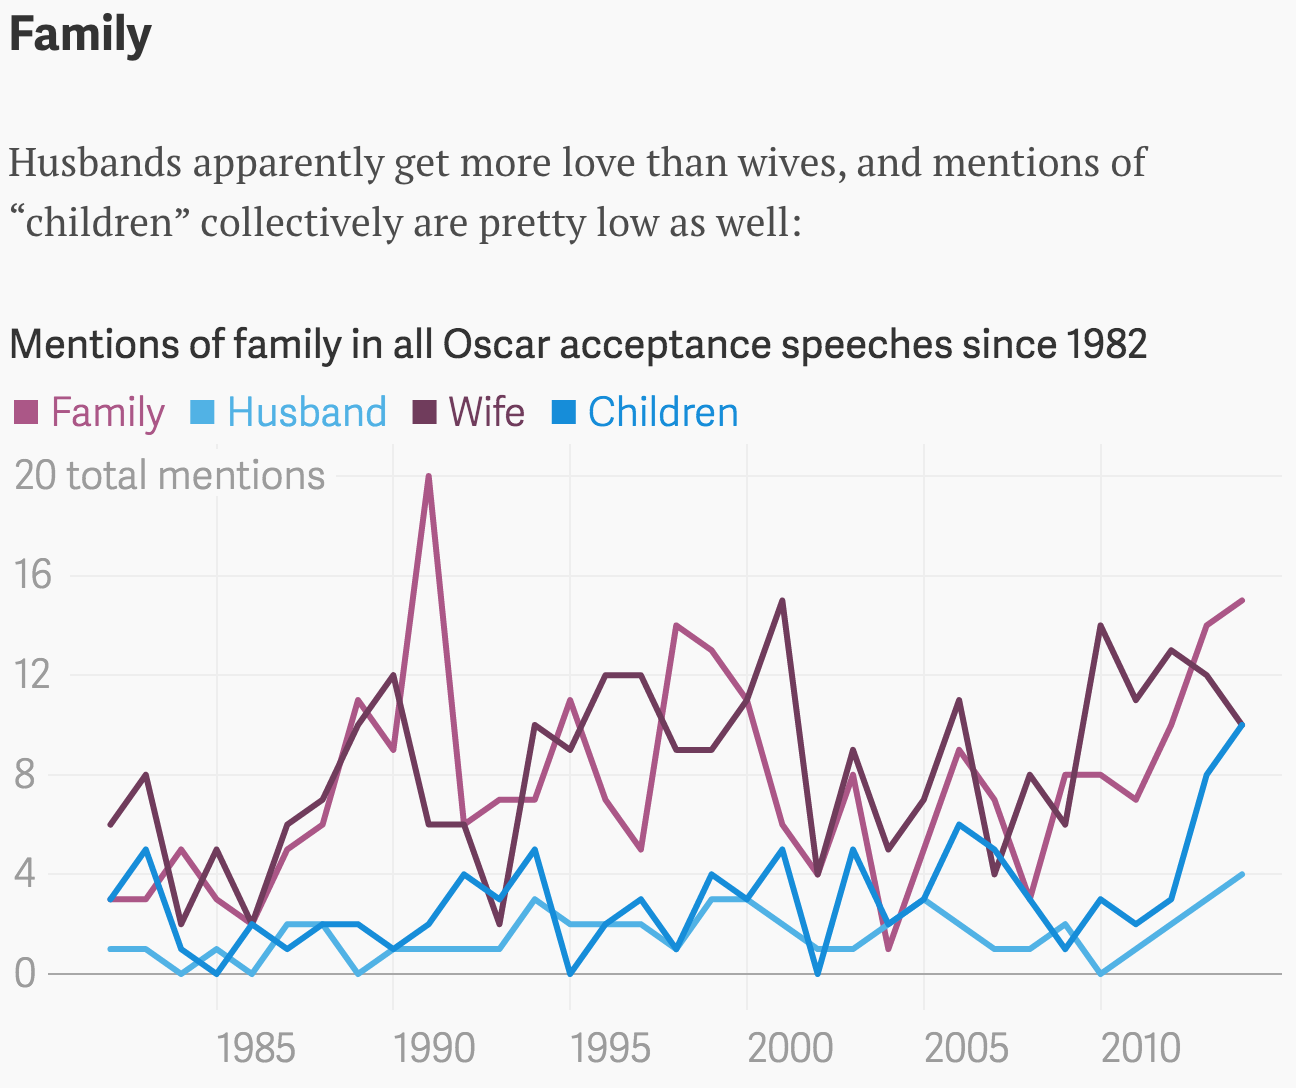
\includegraphics[width=0.7\linewidth]{family.png}
\end{frame}

\begin{frame}\frametitle{Via Quartz:  Who Oscar Winners Thank}
	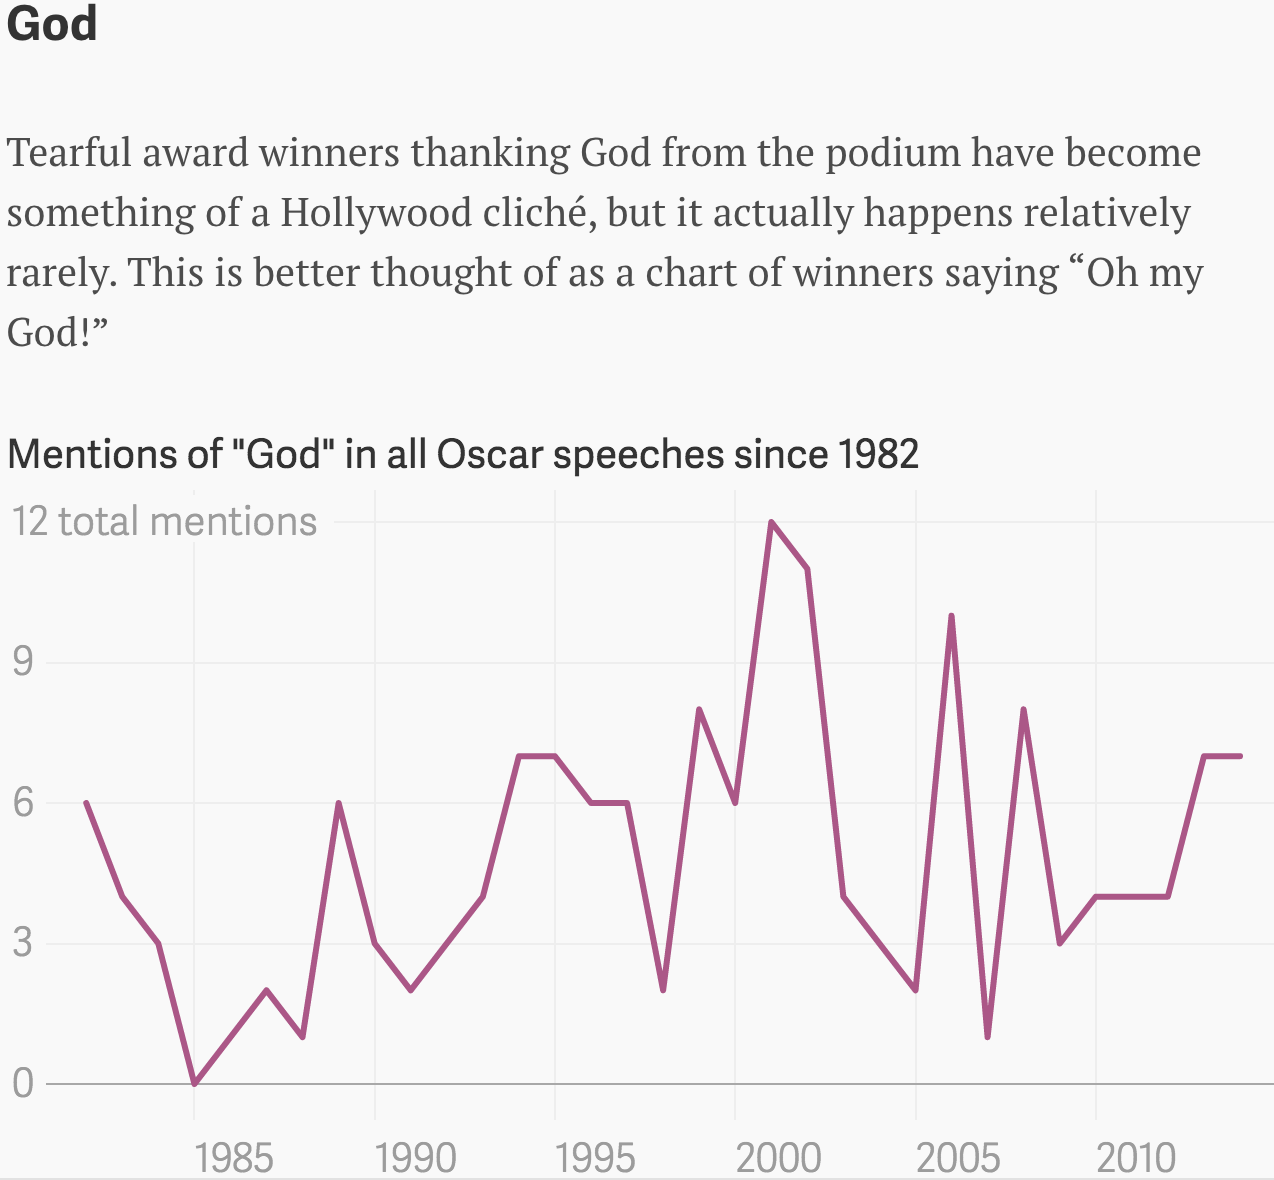
\includegraphics[width=0.7\linewidth]{god.png}
\end{frame}



\begin{frame}\frametitle{``Decorating'' / Data-Ink}
	\small
	
	Graphics should not draw the viewer's attention away from the data.  Extras get in the way.
	
	\vskip 0.25 cm
	
	\textbf{Note:  Decoration does not refer to appropriate graph labeling.}  Labels should always be clear, detailed, and thorough.  \\Label key parts of the data.  Add text explanations if necessary.
	
	\vskip 0.25 cm
	
	\textbf{Data Ink should primarily present information about the data:}  \\the non-erasable, non-redundant core of a graphic
	
	\vskip 0.25 cm
	
	Tufte suggests using the \emph{data-ink ratio}:
	
	\vskip 3 cm
\end{frame}



\begin{frame}\frametitle{``Decorating'' / Data-Ink}
	\small
	
	Two ways to increase the proportion of data-ink:
	
	\vskip 0.25 cm
	
	\textbf{Remove non-data-ink:}  
	
	
	\vskip 2 cm
	
	\textbf{Remove redundant data-ink:} \\ 
	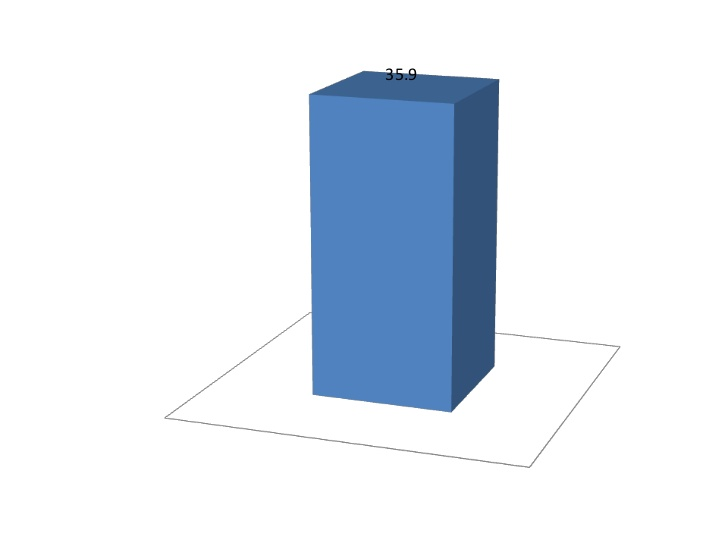
\includegraphics[width = 0.6\linewidth]{data-ink.jpg}
	
	\vskip 3 cm
\end{frame}




\begin{frame}\frametitle{R Package ggplot2 -- Hadley Wickham}
	\small
	
	Based on ``The Grammar of Graphics" by Leland Wilkinson, 2005
	
	\vskip 0.5 cm
	
	ggplot() \# grammar of graphics plot
	
	
	\vskip 0.5 cm
	
	Each plot can be broken down into core components.  Wilkinson defines the core components.  Wickham puts them into practice in R.
	
	\vskip 0.5 cm
	
	Highly recommend these workshop slides:\\https://opr.princeton.edu/workshops/Downloads/2015Jan\_ggplot2Koffman.pdf
\end{frame}



\begin{frame}\frametitle{R Package ggplot2 -- Hadley Wickham}
	\small
	
	
	\begin{enumerate}
		\item \textbf{data}: in ggplot2, data must be stored as an R data frame
		
		\item \textbf{coordinate system}: describes 2-D space that data is projected onto\\
		e.g., Cartesian coordinates, polar coordinates, map projections, ...
		\item \textbf{geoms}: describe type of geometric objects that represent data\\
		e.g., points, lines, polygons, ...
		\item \textbf{aesthetics}: describe visual characteristics that represent data\\
		e.g., for example, position, size, color, shape, transparency, fill
		\item \textbf{scales}: for each aesthetic, describe how visual characteristic is converted to display values\\
		e.g., log scales, color scales, size scales, shape scales, ...
		\item \textbf{stats} : describe statistical transformations that help summarize data\\
		e.g., counts, means, medians, regression lines, ...
		\item \textbf{facets}: describe how data is split into subsets and displayed as multiple small graphs\\
	\end{enumerate}
	
	
\end{frame}


\begin{frame}\frametitle{How Do I Learn ggplot?}
	\small
	
	The best way to learn how ggplot works is through examples!
	
	\vskip 0.5 cm
	
	We'll go through several examples of this in Lab 02 and HW 02
	
	\vskip 2 cm
	
	\large{\textbf{Next Up:  1-D Categorical Data}}
	
	\vskip 0.5 cm
	
	Recall:  Data can be \textbf{categorical} or \textbf{continuous}\\
	
	\vskip 0.5 cm
	
	Categorical data can be \textbf{ordered} or \textbf{unordered / nominal}
	
\end{frame}



\begin{frame}\frametitle{1-D Categorical Data}
	\small
	
	Structure:
	
	\vskip 2.5 cm
	
	How could we summarize this data?\\
	What information would you report?\\
	
	\vskip 10 cm
	
\end{frame}

\begin{frame}\frametitle{1-D Categorical Data}
	\small
	
	To show the differences among the categories, need to use \emph{area plots}:
	
	\vskip 3.5 cm
	
	Examples of area plots?
	
	\vskip 10 cm
	
\end{frame}


\begin{frame}\frametitle{1-D Categorical Data -- Bar Charts}
	\small
	
	\textbf{Bar Charts}:  rectangular bar is created for each unique categorical value.  The area and height of the bar is proportional to \% of observations with the categorical value.  Bars usually have equal width.
	
	
	\vskip 10 cm
	
\end{frame}



\begin{frame}\frametitle{1-D Categorical Data -- Spine Charts}
	\small
	
	\textbf{Spine Charts}:  rectangular bar is created for each unique categorical value.  The height of all bars is equal, and the width of the bar corresponds to the proportion in that category.
	
	\vskip 10 cm
	
\end{frame}



\begin{frame}\frametitle{1-D Categorical Data -- Pie Charts}
	\small
	
	\textbf{Pie Charts}:  circle divided up into sections (``pie slices'') such that the area of each section is proportional to the number of observations with each unique categorical value.
	
	
	\vskip 10 cm
	
\end{frame}


\begin{frame}\frametitle{1-D Categorical Data -- Rose Diagrams}
	\small
	
	\textbf{Rose Diagrams}:  circle sections are created for each category.  All sections have the same width/arc/angle.  The radius is proportional to the square root of the category frequency.  Sections are called ``petals''.  Developed by Florence Nightingale (example will be posted to Blackboard).
	
	
	\vskip 10 cm
	
\end{frame}



\end{document}
